% Fig. 1 of the revised manuscript: closed loop, GRU controller, and the evolutionary
% variational-inference loop. Compile:  pdflatex fig_schematic.tex
\documentclass[border=3pt]{standalone}
\usepackage[T1]{fontenc}
\usepackage{lmodern}
\usepackage{amsmath,amssymb}
\usepackage{tikz}
\usetikzlibrary{arrows.meta,positioning,calc}
\begin{document}
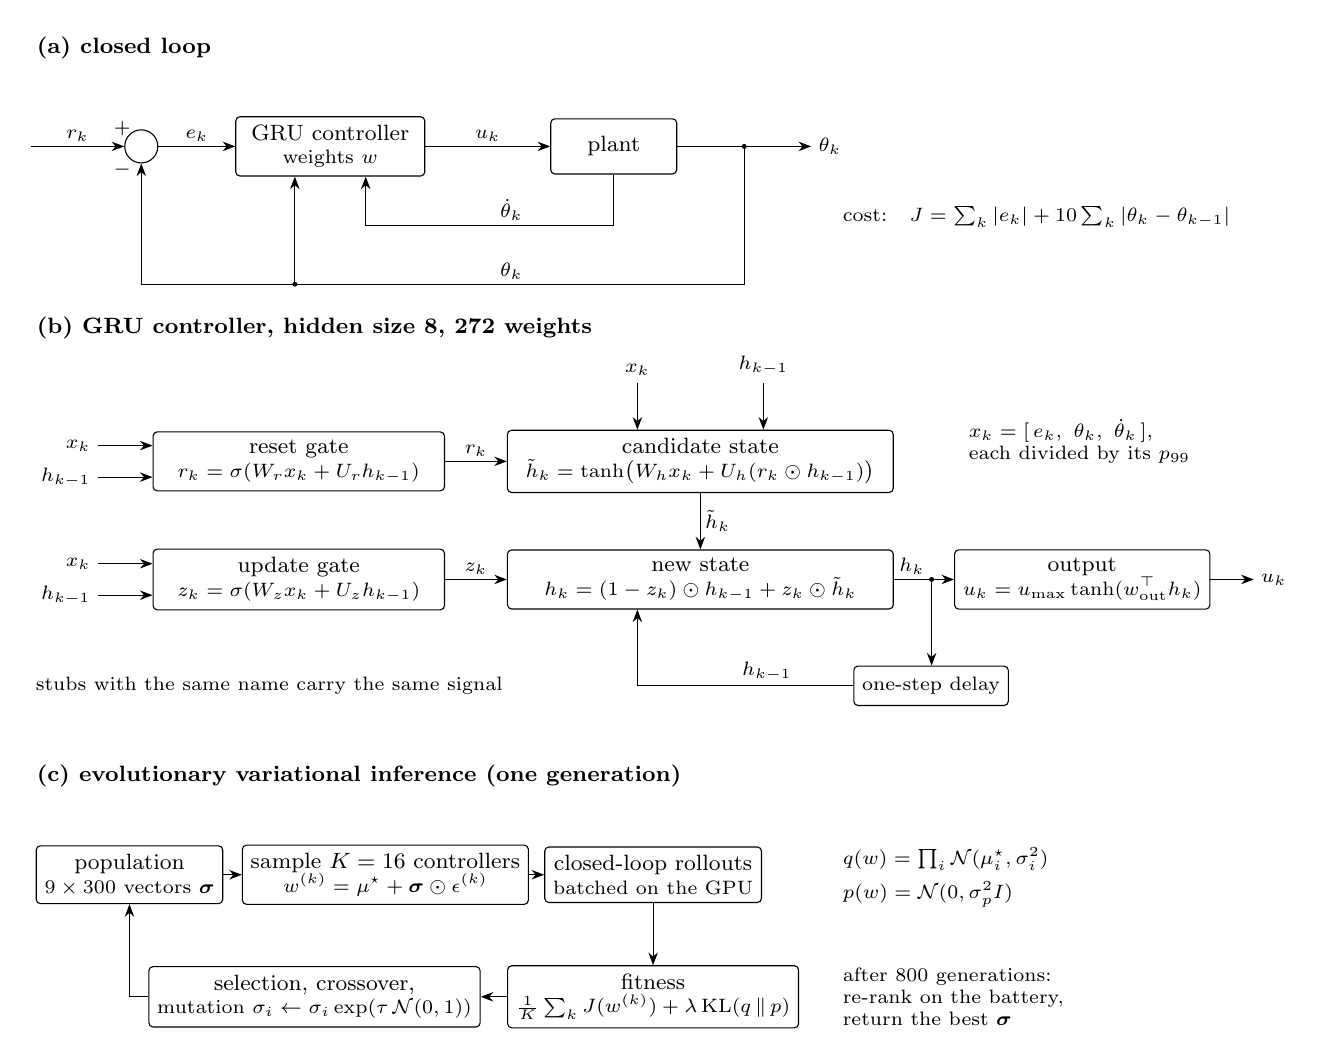
\begin{tikzpicture}[
    font=\footnotesize, >={Stealth[length=1.6mm]},
    box/.style={draw, rounded corners=1.5pt, minimum height=7mm, inner sep=3pt, align=center},
    op/.style={draw, circle, inner sep=0.6pt, minimum size=4.2mm},
    lab/.style={font=\scriptsize, inner sep=1.5pt},
    sig/.style={font=\scriptsize, inner sep=2.5pt},      % signal name at the end of a stub
    panel/.style={font=\footnotesize\bfseries}]

% ================================================================ (a) closed loop
\node[panel, anchor=west] at (-0.55,1.25) {(a) closed loop};
\node[op] (sum) at (0.9,0) {};
\node[lab] at ($(sum)+(-0.24,0.22)$) {$+$};
\node[lab] at ($(sum)+(-0.24,-0.3)$) {$-$};
\node[box, minimum width=24mm] (ctrl) at (3.3,0) {GRU controller\\[-1pt]{\scriptsize weights $w$}};
\node[box, minimum width=16mm] (plant) at (6.9,0) {plant};
\draw[->] (-0.5,0) -- node[lab, above] {$r_k$} (sum);
\draw[->] (sum) -- node[lab, above] {$e_k$} (ctrl);
\draw[->] (ctrl) -- node[lab, above] {$u_k$} (plant);
% controlled variable: the angle
\draw[->] (plant.east) -- ++(1.7,0) node[sig, right] {$\theta_k$};
\coordinate (tap) at ($(plant.east)+(0.85,0)$);
\fill (tap) circle (0.9pt);
% the angle is fed back to the summing junction ...
\draw[->] (tap) |- (0.9,-1.75) -- (sum.south);
\node[lab, above] at (5.6,-1.75) {$\theta_k$};
% ... and is also an input of the controller
\coordinate (tapc) at (2.85,-1.75);
\fill (tapc) circle (0.9pt);
\draw[->] (tapc) -- (tapc |- ctrl.south);
% the rate is measured separately and goes to the controller only
\coordinate (rate) at (3.75,-1.0);
\draw[->] (plant.south) |- (rate) -- (rate |- ctrl.south);
\node[lab, above] at (5.6,-1.0) {$\dot\theta_k$};
% cost, on one line
\node[lab, anchor=west] at (9.75,-0.9)
  {cost:\quad $J=\sum_k |e_k|+10\sum_k|\theta_k-\theta_{k-1}|$};

% ================================================================ (b) GRU controller
\begin{scope}[shift={(0,-4.75)}]
\node[panel, anchor=west] at (-0.55,2.45) {(b) GRU controller, hidden size 8, 272 weights};
\node[box, minimum width=37mm] (R) at (2.9,0.75) {reset gate\\[-1pt]{\scriptsize $r_k=\sigma(W_r x_k+U_r h_{k-1})$}};
\node[box, minimum width=37mm] (Z) at (2.9,-0.75) {update gate\\[-1pt]{\scriptsize $z_k=\sigma(W_z x_k+U_z h_{k-1})$}};
\node[box, minimum width=49mm] (C) at (8.0,0.75) {candidate state\\[-1pt]{\scriptsize $\tilde h_k=\tanh\!\big(W_h x_k+U_h(r_k\odot h_{k-1})\big)$}};
\node[box, minimum width=49mm] (S) at (8.0,-0.75) {new state\\[-1pt]{\scriptsize $h_k=(1-z_k)\odot h_{k-1}+z_k\odot\tilde h_k$}};
\node[box, minimum width=31mm] (O) at (12.85,-0.75) {output\\[-1pt]{\scriptsize $u_k=u_{\max}\tanh(w_{\mathrm{out}}^{\top}h_k)$}};
% inputs of the two gates: one stub per signal
\draw[->] (0.35,0.95)  node[sig, left] {$x_k$}     -- (R.west |- 0,0.95);
\draw[->] (0.35,0.55)  node[sig, left] {$h_{k-1}$} -- (R.west |- 0,0.55);
\draw[->] (0.35,-0.55) node[sig, left] {$x_k$}     -- (Z.west |- 0,-0.55);
\draw[->] (0.35,-0.95) node[sig, left] {$h_{k-1}$} -- (Z.west |- 0,-0.95);
% inputs of the candidate state
\draw[->] (7.2,1.75) node[sig, above] {$x_k$}     -- (7.2,0 |- C.north);
\draw[->] (8.8,1.75) node[sig, above] {$h_{k-1}$} -- (8.8,0 |- C.north);
% signals between the blocks
\draw[->] (R) -- node[lab, above] {$r_k$} (C);
\draw[->] (Z) -- node[lab, above] {$z_k$} (S);
\draw[->] (C) -- node[lab, right] {$\tilde h_k$} (S);
\draw[->] (S) -- node[lab, above, pos=0.3] {$h_k$} (O);
\draw[->] (O.east) -- ++(0.55,0) node[sig, right] {$u_k$};
% recurrence: the new state, delayed by one step, is the old state of the next step
\coordinate (htap) at ($(S.east)+(0.48,0)$);
\fill (htap) circle (0.9pt);
\node[box, minimum height=5mm, minimum width=19mm, font=\scriptsize] (D) at (10.93,-2.1) {one-step delay};
\draw[->] (htap) -- (htap |- D.north);
\draw[->] (D.west) -| node[lab, above, pos=0.2] {$h_{k-1}$} (7.2,0 |- S.south);
% notes
\node[lab, anchor=west, align=left] at (11.35,1.0)
  {$x_k=[\,e_k,\ \theta_k,\ \dot\theta_k\,]$,\\ each divided by its $p_{99}$};
\node[lab, anchor=west] at (-0.5,-2.1) {stubs with the same name carry the same signal};
\end{scope}

% ================================================================ (c) evolutionary VI
\begin{scope}[shift={(0,-9.55)}]
\node[panel, anchor=west] at (-0.55,1.55) {(c) evolutionary variational inference (one generation)};
\node[box, minimum width=21mm] (pop) at (0.75,0.3) {population\\[-1pt]{\scriptsize $9\times300$ vectors $\boldsymbol\sigma$}};
\node[box, minimum width=27mm] (samp) at (4.0,0.3) {sample $K=16$ controllers\\[-1pt]{\scriptsize $w^{(k)}=\mu^{\star}+\boldsymbol\sigma\odot\epsilon^{(k)}$}};
\node[box, minimum width=24mm] (roll) at (7.4,0.3) {closed-loop rollouts\\[-1pt]{\scriptsize batched on the GPU}};
\node[box, minimum width=27mm] (fit) at (7.4,-1.25) {fitness\\[-1pt]{\scriptsize $\tfrac1K\sum_k J(w^{(k)})+\lambda\,\mathrm{KL}(q\,\Vert\,p)$}};
\node[box, minimum width=38mm] (var) at (3.1,-1.25) {selection, crossover,\\[-1pt]{\scriptsize mutation $\sigma_i\leftarrow\sigma_i\exp(\tau\,\mathcal N(0,1))$}};
\draw[->] (pop) -- (samp);
\draw[->] (samp) -- (roll);
\draw[->] (roll) -- (fit);
\draw[->] (fit) -- (var);
\draw[->] (var.west) -| (pop.south);
\node[lab, anchor=west] at (9.75,0.5) {$q(w)=\prod_i\mathcal N(\mu^{\star}_i,\sigma_i^2)$};
\node[lab, anchor=west] at (9.75,0.05) {$p(w)=\mathcal N(0,\sigma_p^2 I)$};
\node[lab, anchor=west, align=left] at (9.75,-1.25) {after 800 generations:\\re-rank on the battery,\\return the best $\boldsymbol\sigma$};
\end{scope}
\end{tikzpicture}
\end{document}
